% \textit{\textbf{The following section formatting is \textbf{optional}, you can also define sections as you deem fit.
% \
% Focus on what future researchers or practitioners would find useful for reproducing or building upon the paper you choose.\
% For more information on our previous challenges, refer to the editorials \citep{Sinha:2022,Sinha:2021,Sinha:2020,Pineau:2019}.
% }}

\newcommand\blfootnote[1]{%
  \begingroup
  \renewcommand\thefootnote{}\footnote{#1}%
  \addtocounter{footnote}{-1}%
  \endgroup
}

\newcommand{\xmark}{\text{\ding{55}}}
\makeatletter
\newcommand\newtag[2]{#1\def\@currentlabel{#1}\label{#2}}
\makeatother
\newcommand*{\eg}{e.g.\@\xspace}
\newcommand*{\ie}{i.e.\@\xspace}

\section{Introduction}
% A few sentences placing the work in a high-level context. Limit it to a few paragraphs at most; your report is on reproducing a piece of work, and you don’t have to motivate that work.

 % Although there is extensive work in this direction, previous work almost exclusively focuses on models obtained in a supervised setting. The problem of extending the Feature Importance and Example Importance methods to an unsupervised setting is the main subject of the paper \textit{Label-Free Explainability for Unsupervised Models}, by J. Crabbé and M. van der Schaar \citep{mainpaper}, which we reproduce in this work.

 % One such model-agnostic, post hoc method treats the model as a black box. The explanation method then explains the predictions of this black box. 
Deep learning models are getting more and more advanced,  making it difficult for humans to understand and retrace how an algorithm arrives at a specific result. To solve this problem, explanation methods were developed.

Post-Hoc methods separate explanations from models allowing explanation methods to be compatible with a variety of models \citep{xaisurvey}. They treat these models as \enquote{black boxes} due to their increasing complexity. Most of the post-hoc explanation techniques require labels to explain black-box outputs and thus they work only in a supervised setting.

The paper \textit{Label-Free Explainability for Unsupervised Models}, by J. Crabbé and M. van der Schaar \citep{mainpaper} 's goal is to explain black-box outputs in a label-free setting. The authors introduce two extensions for the \textbf{Feature Importance} and the \textbf{Example Importance} that highlight influential features and training examples respectively for a black box to construct representations at inference time. 
\\
\\
The contribution of our work is summarized as follows: 
\begin{enumerate}[noitemsep,topsep=0pt]
    \item We reproduce the main experiments by Crabbé and Schaar \citep{mainpaper} to reproduce their main claims.
    \item We conduct additional experiments to assess the robustness of label-free techniques proposed by the authors. Since they originally experiment on image and time-series datasets, we extend their techniques to find salient features and training samples for graphs and text datasets respectively.  
    \item We find that one of the authors' claims is model-specific when we introduce a penalty term to the loss function of those models.
\end{enumerate}

The code implementation of our study is publicly available\footnote{\url{https://github.com/valentinosPariza/Re-Label-Free-XAI}}.

\section{Scope of reproducibility}
% Introduce the specific setting or problem addressed in this work and list the main claims from the original paper. Think of this as writing out the main contributions of the original paper. Each claim should be relatively concise; some papers may not clearly list their claims, and one must formulate them in terms of the presented experiments. (For those familiar, these claims are roughly the scientific hypotheses evaluated in the original work.)

% A claim should be something that can be supported or rejected by your data. An example is, Finetuning pretrained BERT on dataset X will have higher accuracy than an LSTM trained with GloVe embeddings.'' % This is concise, and is something that can be supported by experiments. % An example of a claim that is too vague, which can't be supported by experiments, is Contextual embedding models have shown strong performance on a number of tasks. We will run experiments evaluating two types of contextual embedding models on datasets X, Y, and Z."

% This section roughly tells a reader what to expect in the rest of the report. Clearly itemize the claims you are testing:
% \begin{itemize}
% \item Claim 1
% \item Claim 2
% \item Claim 3
% \end{itemize}

% \item\label{claim3} \textbf{Interpretability} of saliency maps derived from VAE latent units \textbf{is hard} and \textbf{unrelated to the increase in disentanglement} between those latent units.

The original paper provides label-free extensions of feature and example importance methods.  
 We identify the following main claims from the paper:
\begin{enumerate}[labelindent=\parindent,leftmargin=*, label=\textbf{Claim \arabic*},noitemsep,topsep=0pt]
    \itemsep0em
    \item\label{claim1}Label-free \textbf{feature importance} scores allow us to determine salient features of a model's input that contribute to an output prediction.
    \item\label{claim2}Label-free \textbf{example importance} scores allow us to determine salient training examples that explain a test example.
    \item\label{claim3} \textbf{Interpretability} of saliency maps derived from disentangled VAE latent units \textbf{is hard} and is \textbf{unrelated to the strength of disentanglement} between those units.
    \item\label{claim4} Distinct pretext tasks \textbf{don't have interchangeable representations}, and for example importance, pretext tasks with labels have more different representations than label-free pretext tasks.
\end{enumerate}
\  \\
\ref{claim1} and \ref{claim2} are the hypotheses focusing directly on the proposed extensions. \ref{claim3} focuses on the extent of application of \ref{claim1}. \ref{claim4} addresses practical utility of \ref{claim1} and \ref{claim2}. Our additional experiments challenge the robustness of \ref{claim1} and \ref{claim2} and the generalizability of \ref{claim3}.


\section{Methodology}
\label{section:methodology}
% Explain your approach - did you use the author's code, or did you aim to re-implement the approach from the description in the paper? Summarize the resources (code, documentation, GPUs) that you used.

We use the code provided by the authors, with some minor fixes (missing statements to load libraries, and inconsistent function calls) \citep{Jonathan3:online}. The code is well-structured and documented. We extend the authors' work by providing additional experiments and results. We discuss important concepts pertaining to the original paper in Sections \ref{l2lf} and \ref{sec:attrprior} before we discuss technical aspects. 

\subsection{Going from Label to Label-Free Setting}
\label{l2lf} 
For a supervised setting, feature space $\mathcal{X}$ and label space $\mathcal{Y}$, make a black-box model $f: \mathcal{X}\rightarrow \mathcal{Y}$. For label-free setting,
we train an autoencoder model with parameters $\theta \in \Theta$ using label-free loss $\mathcal{L}: \mathcal{X} \times \Theta \rightarrow \mathbb{R}$ on training set $\mathcal{D}_{train} = \{x^n | n \in \mathbb{N}^*\}$, where sample $x^n \in \mathbb{R}^p$. We then treat the encoder as black box $f: \mathcal{X}\rightarrow \mathcal{H}$, that connects $\mathcal{X}$ and latent space $\mathcal{H} \subset \mathbb{R}^{d_H}, d_H \in \mathbb{N}^*$ using encoder parameters $\theta_e$.

\subsubsection{Feature Importance} In a supervised setting, we calculate the weighted importance score $b_i(f,x)$ for every input feature $i \in d_x$ by summing the importance scores across every component of $f$ (for classification, where we output $j$ probabilities of $j$ classes, we sum across $j$ components of $f$). Similarly, for a label-free setting,  we calculate $b_i(f,x)$ by summing importance scores of $d_H$ latent components.

 To calculate the importance scores, the authors use well-known attribution methods (AMs) - Saliency \citep{Saliency}, Integrated Gradients (IG) \citep{IG} and Gradient Shap \citep{shap} which are implemented as part of the open source library, Captum \citep{Captum:online}. 

\subsubsection{Example Importance} \label{ex_theory} A score $c^n$ is assigned to every training example $x^n$ based on it's importance in explaining a test example $x \in \mathcal{X}$. The original paper introduces two families of methods to compute them \citep{mainpaper}:
\begin{enumerate}
\itemsep0em
    \item \textbf{Loss-Based:} This method simulates the shift in loss $\delta^n_{\theta}\mathcal{L}$ for a test example $x$ when a particular training example $x^n$ is removed. The $\delta^n_{\theta}\mathcal{L}$ is also defined as the score $c^n$ for $x^n$. In a supervised setting, we utilize the data label $y^n$ to evaluate the loss for the entire model. But in a label-free setting, we only rely on the representations from the encoder and drop the decoder. Hence, we also decompose overall parameter gradients as relevant (encoder) and irrelevant (decoder). We only consider shifts in the loss by relevant parameters. This is done by differentiating the loss $\mathcal{L}$ with respect to $\theta_e$.
    \item \textbf{Representation-Based:} This method assigns a score by analyzing latent representations of training examples. In a supervised setting, we consider representations as the output of an intermediate layer $f_e(x)$. The similarity between the representation of test and training set examples can be quantified by reconstructing $f_e(x)$ with $f_e(\mathcal{D}_{train}): f_e(x) \approx \sum_{n=1}^N w^n(x) \cdot f_e(x^n)$. The weight $w^n(x)$ is defined as the score $c^n$ for $x^n$. For a label-free setting, we use encoder output, $f_e(x)$.
\end{enumerate}

For loss-based, the authors use the Influence Function \citep{Koh} and TracIn \citep{Pruthi} AMs. And for representation-based, the authors introduce two AMs - DKNN and SimplEx \citep{mainpaper}.

% An importance score $c^n(f,x)$ is calculated for every training example $x^n$ to construct a representation of a test example $x \in \mathcal{X}$ using black-box $f(x) \in \mathcal{H}$. The original paper introduces two families of methods to compute them \citep{mainpaper}:
% \begin{enumerate}
% \itemsep0em
%     \item \textbf{Loss-Based:} The score of each training example is derived from the shift in loss when the example is removed. This shift is calculated using two methods - Influence Function \citep{Koh} and TracIn \citep{Pruthi} by differentiating the loss $\mathcal{L}$ with respect to $\Theta_e$.
%     \item \textbf{Representation-Based:} The score is assigned by taking a weighted sum of the latent representations of training examples $\sum_{n=1}^N w^n(x). f(x^n)$ to reconstruct latent representation of test example $f(x)$. The weights $w^n(x)$ are the importance scores $c^n$, calculated using two methods - DKNN and Simplex \citep{mainpaper}. 
% \end{enumerate}

\subsection{Additional Experiments: Attribution Priors}
\label{sec:attrprior}
Attribution prior encodes domain knowledge into a model \citep{attrprior}. The prior knowledge is defined by a function $\Omega:\mathbb{R}^{p\times n}\rightarrow\mathbb{R}$ that gets an attribution matrix $\Phi$. In this work, we use pixel attribution prior which is a penalty function on pixel attributions, that promotes a high level of smoothness in the attributions by minimizing the total variation of neighbouring pixel attributions. It was introduced by Erion et al. \citep{attrprior} and is defined as:
\begin{align}\label{eqn:pixelattrprior}
    \Omega_{pixel}(\Phi(\theta,\mathcal{X})) = \sum_{l}\sum_{i,j}{|\phi_{i+1,j}^l-\phi_{i,j}^l|+|\phi_{i,j+1}^l-\phi_{i,j}^l|}
\end{align}
Here, $\phi_{i,j}^l$ is the attribution of $i,j$-th pixel for $l$-th training sample. Encoding prior knowledge of the model is done by adding $\Omega$ to the model's loss function:
\begin{align}\label{eqn:losswithattrprior}
\theta^* = \argmin_\theta \mathcal{L}(\theta; \mathcal{X}, y)+ \lambda\Omega(\Phi(\theta, \mathcal{X}))
\end{align}
\subsection{Model descriptions}
\label{model_descriptions}
% Include a description of each model or algorithm used. Be sure to list the type of model, the number of parameters, and other relevant info (e.g. if it's pretrained). 
We use the same models as used by the authors, except for the text and variational graph autoencoder. Table \ref{tab:modeloverview} gives an overview of the models used. We train these models and use the trained models during inference to find salient features and training samples.

\begin{table}[H]
    \small
    \centering
    \begin{tabular}{lllll}
    \toprule
     \textbf{Model} & \textbf{Input Dataset} & \textbf{\# of Params} & \textbf{Evaluated Claims}\\
    \midrule 
    \multirow{2}{*}{CNN Denoising Autoencoder$^*$} & MNIST & 87.1k  &  \hyperref[claim1]{1}, \hyperref[claim2]{2},  \hyperref[claim4]{4} \\
        &     Tiny ImageNet & 416.3k &  \hyperref[claim1]{1}, \hyperref[claim2]{2}\\
    \midrule   
    LSTM Reconstruction Autoencoder &  ECG5000 & 249.4k & \multirow{2}{*}{\hyperref[claim1]{1}, \hyperref[claim2]{2}}  \\
    SimCLR & CIFAR-10 & 12481.7k  \\
    \midrule
      \multirow{2}{*}{$\beta$-VAE$^*$ \& TC-VAE$^*$} & MNIST & 463.7k  & \multirow{2}{*}{\hyperref[claim3]{3}} \\
        &     dSprites & 502k & \\ 
    \midrule
    Text Autoencoder$^*$  & AGNews & 4048.1k &  \hyperref[claim2]{2}\\
    Variational Graph Autoencoder$^*$  & Cora & 46.8k &  \hyperref[claim1]{1} \\

    \bottomrule
    \end{tabular}
    \caption{Overview of models used. $^*$ denotes models used for additional experiments. We use MNIST's autoencoder model for Tiny ImageNet with the input size set to 64 and $d_H=16$.}
    \label{tab:modeloverview}
\end{table}


\subsection{Datasets}
% For each dataset include 1) relevant statistics such as the number of examples and label distributions, 2) details of train / dev / test splits, 3) an explanation of any preprocessing done, and 4) a link to download the data (if available).
% Say a few words about the datasets and specifically about the tasks our experiments were conducted on. Use this space to refer to the table below. Say that we use the same datasets but also we use a few extra datasets for our additional experiments. Describe the new datasets since they have not been described in the original paper.

 The original paper's experiments generate latent representations for the black-box models.  Table \ref{tab:modeloverview} denotes which dataset was used to train which model. Table \ref{tab:dataset} provides an overview of these datasets. The authors use MNIST, ECG5000, CIFAR-10, and dSprites datasets in their experiments. Tiny ImageNet is a subset of the ImageNet dataset \citep{ImageNet18:online}. We use Tiny ImageNet to see whether \ref{claim1} and \ref{claim2} are satisfied on an image dataset other than the ones used by authors. Cora dataset consists of academic publications as nodes and citations between them as links. We use the Cora dataset to explain graphs in a label-free setting. For text explainability, we take a balanced subset of the AGNews dataset while normalizing and tokenizing the text, keeping a maximum token length of 64 \citep{agnewspaper}.
% {l|cc|c|cc}
\begin{table}[h]
    \small
    \centering
    \begin{tabular}{lcccl}
    \toprule
    \multirow{2}{*}{\textbf{Dataset}} & \multicolumn{2}{c}{\textbf{Samples}} & \multirow{2}{*}{\textbf{Classes}} & \multirow{2}{*}{\textbf{Description}}\\
    & \textbf{Training} & \textbf{Test} \\
    \midrule 
    MNIST$^*$ &  60K &  10K & 10 &  28x28 grayscale images of the digits \citep{MNIST—To58:online}  \\
    ECG5000 & 4K & 1K & 2 & Time Series - 20 hour long ECG \citep{TimeSeri77:online}  \\
    CIFAR-10$^*$ & 50K & 10K & 10 & 32x32 colour images \citep{CIFAR10—84:online}  \\
    dSprites$^*$\Cross & 73K & n/a & 6 &  64x64 grayscale images of 2D shapes \citep{dsprites17} \\
    Tiny ImageNet$^*$ & 100K & 10K & 200 & 64×64 colour images \citep{TinyImag26:online} \\
    AGNews$^*$ & 10K & 1.7K & 4 & Collection of news articles \citep{AGNews:online} \\
    \toprule
    & Nodes & Edges & \\
    Cora$^*$ &  2708 & 5429 & 7 & Graph Based Citation Network. \citep{cora} \\
    \bottomrule
    \end{tabular}
    \caption{Overview of datasets used. \Cross - 2D shapes in the dataset were generated from six independent latent factors. $*$ - datasets used for additional experiments.}
    \label{tab:dataset}
\end{table}

\subsection{Hyperparameters}
% Describe how the hyperparameter values were set. If there was a hyperparameter search done, be sure to include the range of hyperparameters searched over, the method used to search (e.g. manual search, random search, Bayesian optimization, etc.), and the best hyperparameters found. Include the number of total experiments (e.g. hyperparameter trials). You can also include all results from that search (not just the best-found results).

% We used the same hyperparameters as the original paper's authors when they were specified, and default parameters from the original implementation when they were not mentioned in the paper. We assumed these default parameters were used in the experiments described in the paper. 

% for the CNN autoencoder used to train on the Tiny Imagenet dataset, in order to incorporate increased input feature complexity
We use the same hyperparameters for all the experiments as the original paper \citep{mainpaper}. The hyperparameters for graph and text explainability are mentioned in the Appendix Sections \ref{sssec:graphmodel} and \ref{sssec:textmodel} respectively.

% Thus, we provide a secondary objective for the SM, to the model that helps tune the model's attention
\subsection{Experimental setup and code}\label{sec:expsetup}
We closely follow the setup of the original paper to reproduce their results \citep{mainpaper}. We reproduce our claims quantitatively using the metrics described in Table \ref{tab:metricsoverview}.  
We mask important pixels to find salient features in images. Likewise, we mask edges and isolate important nodes to find salient nodes in graphs. The setup for graph and text explainability is detailed in Appendix Sections \ref{appendix:graphexplain} and \ref{appendix:textexplain} respectively. 

The authors' \ref{claim3} addresses interpretability for disentangled VAE (d-VAE) models. The claim is based on experiments with \underline{\textbf{two d-VAE}} models, $\beta$-VAE and TC-VAE. We extend this original setup to examine whether \enquote{interpretability is indeed hard} for these two d-VAE models. Ideally, we want to make each latent unit of our d-VAEs pay attention to distinct parts of the input. We attempt to do that by controlling their SM. Thus, we provide a secondary objective for the SM that helps tune the model's attention. This secondary objective is achieved through the use of attribution priors (Section \ref{sec:attrprior}).
 We use the penalty function of pixel attribution prior (Equation \ref{eqn:pixelattrprior}) for d-VAE ($\beta$ and TC) models. We keep $d_H=3$ for MNIST. We train both these d-VAE models with loss $\mathcal{L}$  as in Equation \ref{eqn:losswithattrprior},  $\beta\in \{1,5,10\}$ and regularization parameter, $\lambda \in \{0.001, 0.005, 0.01, 0.1\}$. We select the pixel attribution prior because it works very well \citep{attrprior}. It is simple and easy to compute.

\begin{table}[H]
    \small
    \centering
    \begin{tabular}{lcc}
    \toprule
     \textbf{Experiment} & \textbf{Metric(s)} & \textbf{Description} \\
    \midrule 
    Feature & Latent & Shift:
     $||f(x)-f(m \odot x + (1-m)\odot\Bar{x}||_\mathcal{H}$   \\
    Importance & shift & is calculated for each feature $x_i$ while \\
        & & masking $M$ important features with mask $m$. \\
    \midrule   
    Example & Similarity & The mean correct prediction $\sum_{n=1}^M \delta_{y,y^{n}}/M$ \\
    Importance & Rate & of labels of $M$ most important training \\
        & & examples $y^n$ against label of test example $y$. \\
    \midrule
    Comparison b/w & Pearson & Measures correlation between importance scores \\
    saliency maps & Correlation & by taking covariance between them and dividing \\
        & & by the product of their standard deviations.  \\
    \bottomrule
    \end{tabular}
    \caption{Overview of metrics used.}
    \label{tab:metricsoverview}
\end{table}

% Appendix section \ref{appendix:graphexplain} explains the experimental setup for verifying claims for the task of label-free graph explainability. The setup for handling text data (of AG News dataset) is further described in Appendix section \ref{appendix:textexplain}

\subsection{Computational requirements}
We carried out our experiments on a cluster of nodes, each had an NVIDIA Titan RTX GPU. Our reproducibility study required a total of 110 GPU hours, 90 for the original and 20 for the additional experiments (see Appendix \ref{appendix:computationalcosts} for more information).

\section{Results}
\label{section:results}
% Start with a high-level overview of your results. Do your results support the main claims of the original paper? Keep this section as factual and precise as possible, and reserve your judgement and discussion points for the next "Discussion" section. 


\subsection{Results reproducing original paper}
% For each experiment, say 1) which claim in Section~\ref{section:claims} it supports, and 2) if it successfully reproduced the associated experiment in the original paper. 
% For example, an experiment training and evaluating a model on a dataset may support a claim that that model outperforms some baseline.
% Logically group related results into sections. 

\subsubsection{Claim 1: Label-Free Feature Importance}
\label{sssec:result1}
\ref{claim1} breaks into 4 sub-claims as follows:
\begin{enumerate}[labelindent=\parindent,leftmargin=*, topsep=0pt]
    \itemsep-0.2em
    \item\label{th:first} Latent shift increases sharply for perturbing a few most important features.
    \item \label{th:second}This increase decreases when we disturb less relevant pixels.
    \item \label{th:third}Latent shift by feature-attribution methods is higher than that generated by perturbing random pixels.
    \item \label{th:fourth} Integrated Gradients (IG) outperforms other methods.
\end{enumerate}

Figure \ref{fig:labelfree} shows the trends of latent shifts by 3 AMs - IG, Saliency, and Gradient Shap for 3 black-box models. \textbf{The above 4 sub-claims are reproducible} verifying the reproducibility of 
\ref{claim1} for \textbf{MNIST and ECG5000}. For CIFAR-10, sub-claim \ref{th:third} is not reproducible. We see this discrepancy in Figures \ref{fig:cifar10} and \ref{fig:cifar10their}. We discuss why is that so in Section \ref{sec:discussion}. 
 

\subsubsection{Claim 2: Label-Free Example Importance}
\label{exampleimpresult}
We get the similarity rates for the three datasets by varying the number of selected important training examples, as shown in Figure \ref{fig:labelfreece}. The downward trend of similarity rates indicates that similar training examples are assigned higher importance scores. We also observe that representation-based example importance methods give much higher similarity measures for important training examples than loss-based methods. These results validate the consistency of the example importance methods and we reproduce \ref{claim2}.


\begin{figure*}[!h]
\centering
\begin{subfigure}[b]{0.24\linewidth}
\includegraphics[width=\textwidth]{images/feature_imp/mnist.png}
\caption{MNIST}\label{fig:mnist}
\end{subfigure}
\begin{subfigure}[b]{0.24\linewidth}
\includegraphics[width=\textwidth]{images/feature_imp/ecg5000.png} 
\caption{ECG5000}\label{fig:ecg5000}
\end{subfigure}
\begin{subfigure}[b]{0.24\linewidth}
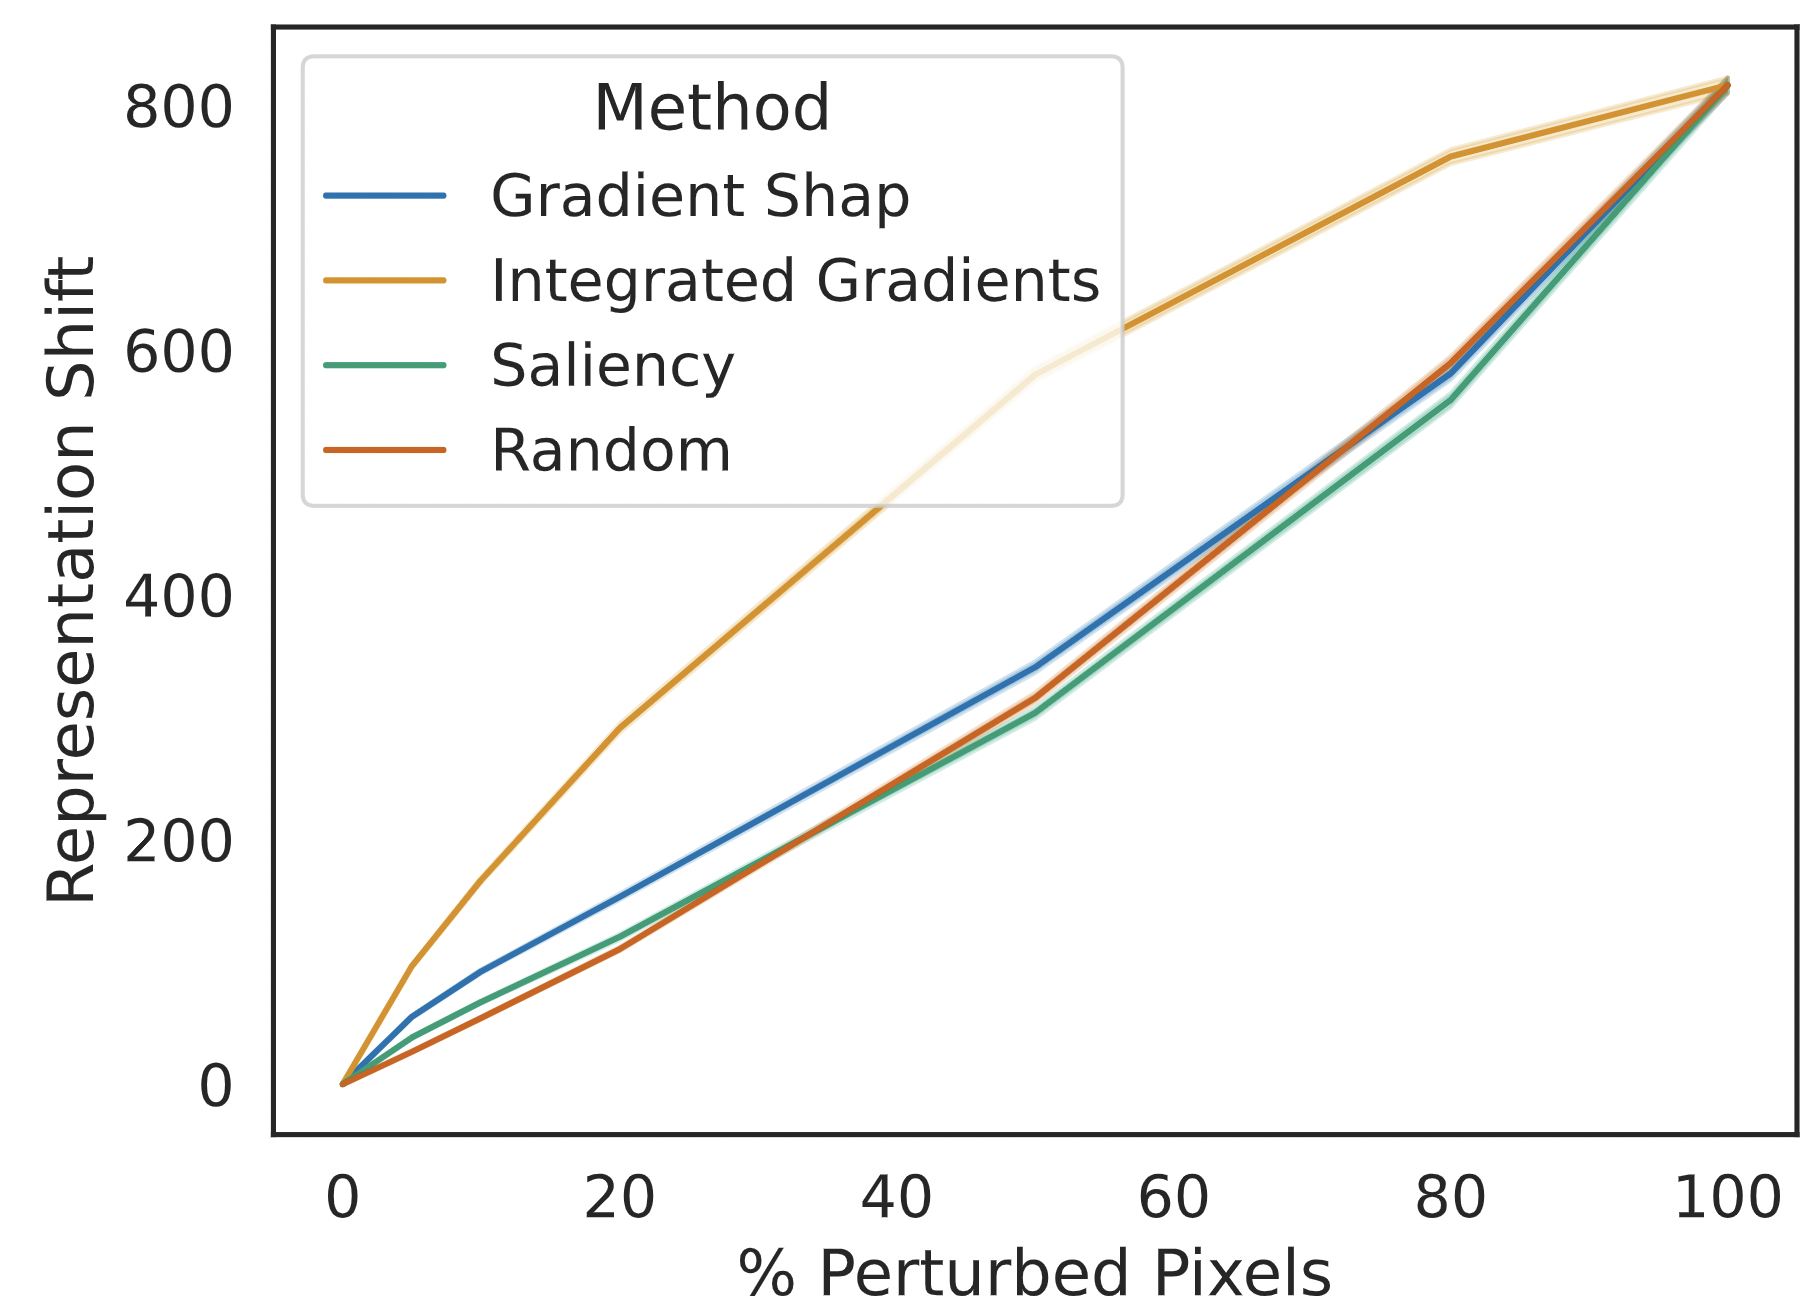
\includegraphics[width=\textwidth]{images/feature_imp/cifar10.png} 
\caption{CIFAR-10 (ours)}\label{fig:cifar10}
\end{subfigure}
\begin{subfigure}[b]{0.24\linewidth}
\includegraphics[width=\textwidth]{images/feature_imp/cifar10_theirs.png} 
\caption{CIFAR-10 (theirs)}\label{fig:cifar10their}
\end{subfigure}
\caption{Consistency check for label-free feature importance.}\label{fig:labelfree}
\end{figure*}

\begin{figure*}[h]
\centering
\begin{subfigure}[b]{0.24\linewidth}
\includegraphics[width=\textwidth]{images/example_imp/mnist_repr.png}
\caption{MNIST}\label{fig:mnistce}
\end{subfigure}
\begin{subfigure}[b]{0.24\linewidth}
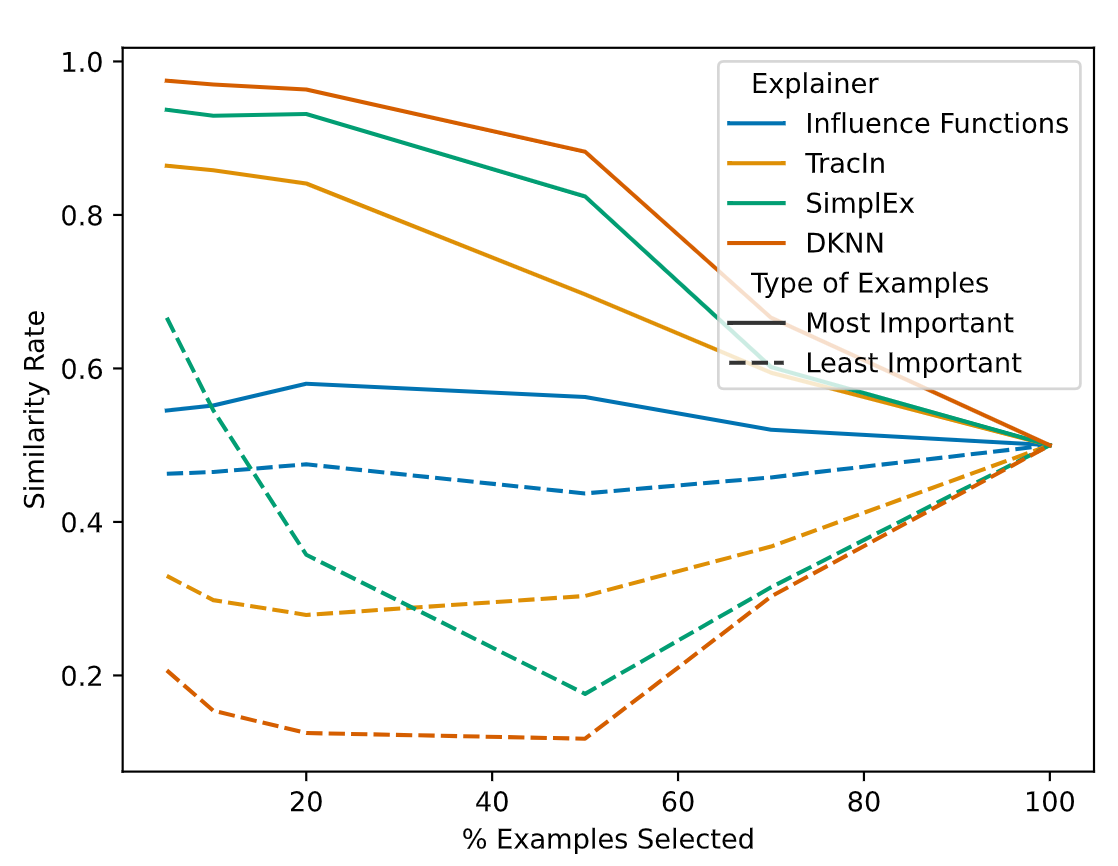
\includegraphics[width=\textwidth]{images/example_imp/ecg_repr.png} 
\caption{ECG5000}\label{fig:ecg5000_ce}
\end{subfigure}
\begin{subfigure}[b]{0.24\linewidth}
\includegraphics[width=\textwidth]{images/example_imp/cifar_res18_repr.png} 
\caption{CIFAR-10}\label{fig:cifar10_ce}
\end{subfigure}
\caption{Consistency check for label-free example importance.}\label{fig:labelfreece}
\end{figure*}

% The authors state that sub-claims \ref{res3:sub1} and \ref{res3:sub2} are applicable only for $\beta$-VAE and TC-VAE models and do not apply in general.
\subsubsection{Claim 3: Latent Space Interpretability of Disentangled VAEs using saliency maps (SM)}\label{section:result3}
We break \ref{claim3} into two sub-claims: 

\begin{enumerate}[labelindent=\parindent,leftmargin=*, topsep=0pt]
    \itemsep-0.2em
    \item\label{res3:sub1} Interpretation and association of the d-VAE model's latent units with clear generative factors is hard using their saliency maps (SM).
    \item \label{res3:sub2}  Interpretations with SM cannot be improved with the increase in disentanglement between the latent units. 
\end{enumerate}

 We examine the SM of each model's encoder's latent units to verify these two sub-claims.

\textbf{Qualitative Result}: We observe that a latent unit is sensitive to a given image while insensitive to a similar image (Figure \ref{fig:qualitativevaemnist}, Image 1 versus Image 2 for latent unit 1). The latent unit's focus changes completely between two similar images (Figure \ref{fig:qualitativevaedsprites}, Image 1 versus Image 2 for latent unit 5). Several latent units focus on the same part of the image (Image 3 of Figures \ref{fig:qualitativevaemnist} and \ref{fig:qualitativevaedsprites}). These observations agree with the authors' observations and support sub-claim \ref{res3:sub1}. Figures \ref{fig:tcvae1smsdsprites} to \ref{fig:betavae10smsmnist2} present the full list of SM used for comparisons. 

\textbf{Quantitative Result}: Figure \ref{fig:mnistvaebox}  shows that when we increase the disentanglement factor $\beta$, it does not lead to a strong increase in decorrelation between the SM of different latent units. Consequently, this suggests that SM are not appropriate for distinguishing generative factors of latent units of d-VAEs, thus proving sub-claims \ref{res3:sub1} and \ref{res3:sub2}.

Hence, our results agree with those of the authors; thus \textbf{\ref{claim3} is reproducible.}

\begin{figure*}[b!]
\centering
\begin{subfigure}[b]{0.32\linewidth}
\includegraphics[width=\textwidth]{images/vae/metric_box_plots_mnist.PNG}
\caption{MNIST}\label{fig:mnistvaebox}
\end{subfigure}
\begin{subfigure}[b]{0.32\linewidth}
\includegraphics[width=\textwidth]{images/vae/metric_box_plots_dSprites.PNG} 
\caption{dSprites}\label{fig:dspritesvaebox}
\end{subfigure}
\begin{subfigure}[b]{0.32\linewidth}
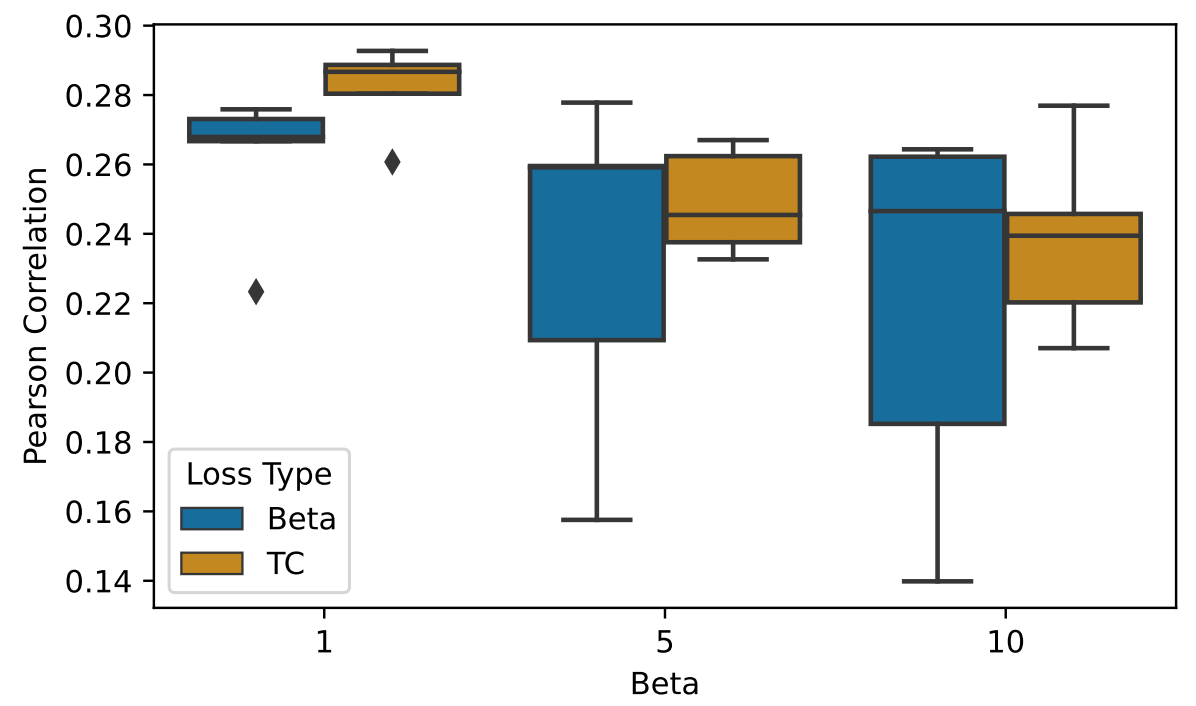
\includegraphics[width=\textwidth]{images/vae/metric_box_plots_mnist_0_005.PNG}
\caption{MNIST ($\lambda= 0.005$ )}\label{fig:mnistvaeboxattrpr}
\end{subfigure}
\caption{PCC over pairs of saliency maps (Gradient Shap) from each combination of a model's latent unit for different values of β. Figure \ref{fig:mnistvaeboxattrpr} uses attribution priors as explained in Section \ref{sec:expsetup}. }\label{fig:vaeboxes}
\end{figure*}


\begin{figure*}[b!]
\centering
\begin{subfigure}[b]{0.35\linewidth}
\includegraphics[width=\textwidth]{images/vae/qualitative_vae_mnist.png}
\caption{MNIST ($\beta$-VAE with $\beta$=10)}\label{fig:qualitativevaemnist}
\end{subfigure}
\begin{subfigure}[b]{0.60\linewidth}
\includegraphics[width=\textwidth]{images/vae/qualitative_vae_dsprites.png} 
\caption{dSprites (TC-VAE with $\beta$=1)}\label{fig:qualitativevaedsprites}
\end{subfigure}
\caption{Saliency maps for each latent unit of the disentangled VAEs. The VAES selected were the ones with the lowest PCC. $i^{th}$ saliency dimension highlights latent unit $i$.} 
\end{figure*}

% In the case of feature importance, the PCCs have values similar to that of the fixation of two human subjects (two human subjects give two different observations) \citep{Ouerhani2003EmpiricalVO} and therefore each pretext task focuses on different features. For example importance, the difference in example representations is even more acute.
\subsubsection{Claim 4: Comparing the learned Pretext Tasks Representations}\label{section:result4}
We break \ref{claim4} into 3 sub-claims and also discuss the respective results of each of the sub-claims as follows:
\begin{enumerate}[labelindent=\parindent,leftmargin=*, topsep=0pt]
    \itemsep-0.2em
\item \textbf{Distinct pretext tasks do not yield interchangeable explainability representations}. We see in Table \ref{tab:tablea} that the Pearson Correlation Coefficients (PCCs) for \textbf{feature importance} range between 0.32 and 0.44 (\textbf{moderate positive correlation}). PCCs range between 0.06 and 0.13 (\textbf{weak positive correlation}) for \textbf{example importance} (Table \ref{tab:tableb}).   These are in accordance with the original paper and confirm the reproducibility of the first sub-claim. 
\item For feature importance, \textbf{the correlation between label-free pretext tasks' SM and classification tasks' SM is similar to the correlation between SM of label-free pretext tasks}. We see in Table \ref{tab:tablea} that the PCCs between SM of classification and the other label-free pretext tasks are in the same range as the correlations between SM of only the label-free pretext tasks. Thus, we confirm the reproducibility of the second sub-claim.
\item For example importance, \textbf{the correlation  between representations of label-free pretext tasks and the classification task is lower to the correlation between representations of only label-free pretext tasks}. As seen in Table \ref{tab:tableb} the autoencoder-classifier correlations are the lowest, whilst the autoencoder-autoencoder PCCs are higher, as in the original paper.  Hence, the third sub-claim is also reproduced.
\end{enumerate}
The analysis of qualitative results is present in Appendix Section \ref{app:qualitativeanalysis}.


\renewcommand{\arraystretch}{1.2}
\begin{table}[h]
\begin{subtable}{.5\linewidth}
\resizebox{\textwidth}{!}{
\begin{tabular}{|c|ccc|}
\hline
                & \textbf{R}   & \textbf{D}      & \textbf{I}       \\
\hline
 \textbf{D}      & $0.41 \pm 0.02$  &                   &                                      \\
 \textbf{I}     & $0.33 \pm 0.03$  & $0.32 \pm 0.01$ &                                      \\
 \textbf{C} & $0.44 \pm 0.02$  & $0.41 \pm 0.02$ & $0.33 \pm 0.02$                     \\
\hline
\end{tabular}
}
\caption{Saliency maps (avg $\pm$ std).}
\label{tab:tablea}
    \end{subtable}%
    \begin{subtable}{.5\linewidth}
    \resizebox{\textwidth}{!}{
    \begin{tabular}{|c|ccc|}
\hline
                & \textbf{R}   & \textbf{D}      & \textbf{I}       \\
\hline
 \textbf{D}      & $0.09 \pm 0.02$ &   &                                    \\
 \textbf{I}     & $0.13 \pm 0.03$  & $0.1 \pm 0.03$ &                       \\
 \textbf{C} & $0.09 \pm 0.03$  & $0.06 \pm 0.03$ & $0.09 \pm 0.02$ \\
\hline
\end{tabular}
}
\caption{Example Importance (avg $\pm$ std).}
\label{tab:tableb}
    \end{subtable} 
   \caption{Pearson Correlation. R-Reconstruction, D-Denoising, I-Inpainting, C-Classification } 
   \label{tab:pearson_cc_pretext}
\end{table}
\renewcommand{\arraystretch}{1}

\subsection{Results beyond original paper}
% Often papers don't include enough information to fully specify their experiments, so some additional experimentation may be necessary. For example, it might be the case that batch size was not specified, and so different batch sizes need to be evaluated to reproduce the original results. Include the results of any additional experiments here. Note: this won't be necessary for all reproductions.

\subsubsection{Label Free Feature Importance}
\label{sec:result1extra}
% \begin{enumerate}\label{sec:result1extra}
%     \itemsep-0.2em
%     \item Performance on (Out Of Distribution) OOD Datasets:
    We verify whether the 4 sub-claims from Section \ref{sssec:result1} hold for Tiny ImageNet and Cora datasets.
    \textbf{Tiny Imagenet satisfies Claim \ref{th:first}} as seen in Figure \ref{fig:tinyimgnet}. \textbf{For Cora, sub-claims \ref{th:third} and \ref{th:fourth} are not reproducible} as seen in Figure \ref{fig:cora}. Graphs have complicated spatial features (nodes, edges, sub-graphs) which aren't well explained by AMs. This is because AMs rely heavily on computing gradients  which causes \textbf{gradient saturation} on discrete values of the adjacency matrix of graph \citep{gnnpaper}. 
    From these results, we conclude that the approach of generating latent shifts to compute feature importance works  well for images and time-series data. AMs fail to explain graphs well. 
    
\subsubsection{Label Free Example Importance}\label{sec:result2extra}
The results obtained for the Tiny Imagenet dataset shown in Figure \ref{fig:tinyimgnetce} are consistent and similar to the results obtained in the case of MNIST in Figure \ref{fig:mnistce} and satisfy \ref{claim2}. We  observe a declining trend for similarity rate in the case of AGNews' text dataset for Figure \ref{fig:agnews} implying correct assignment of importance scores for most similar training examples. The trends verify that representation-based methods work better than loss-based methods but in the case of a higher percentage of training examples selected, the SimplEx method (representation-based) declines rapidly in performance compared to loss-based methods.

\begin{figure}[!htb]
    \centering
    \begin{minipage}{.98\textwidth}
        \centering
        \begin{subfigure}[b]{0.24\linewidth}
            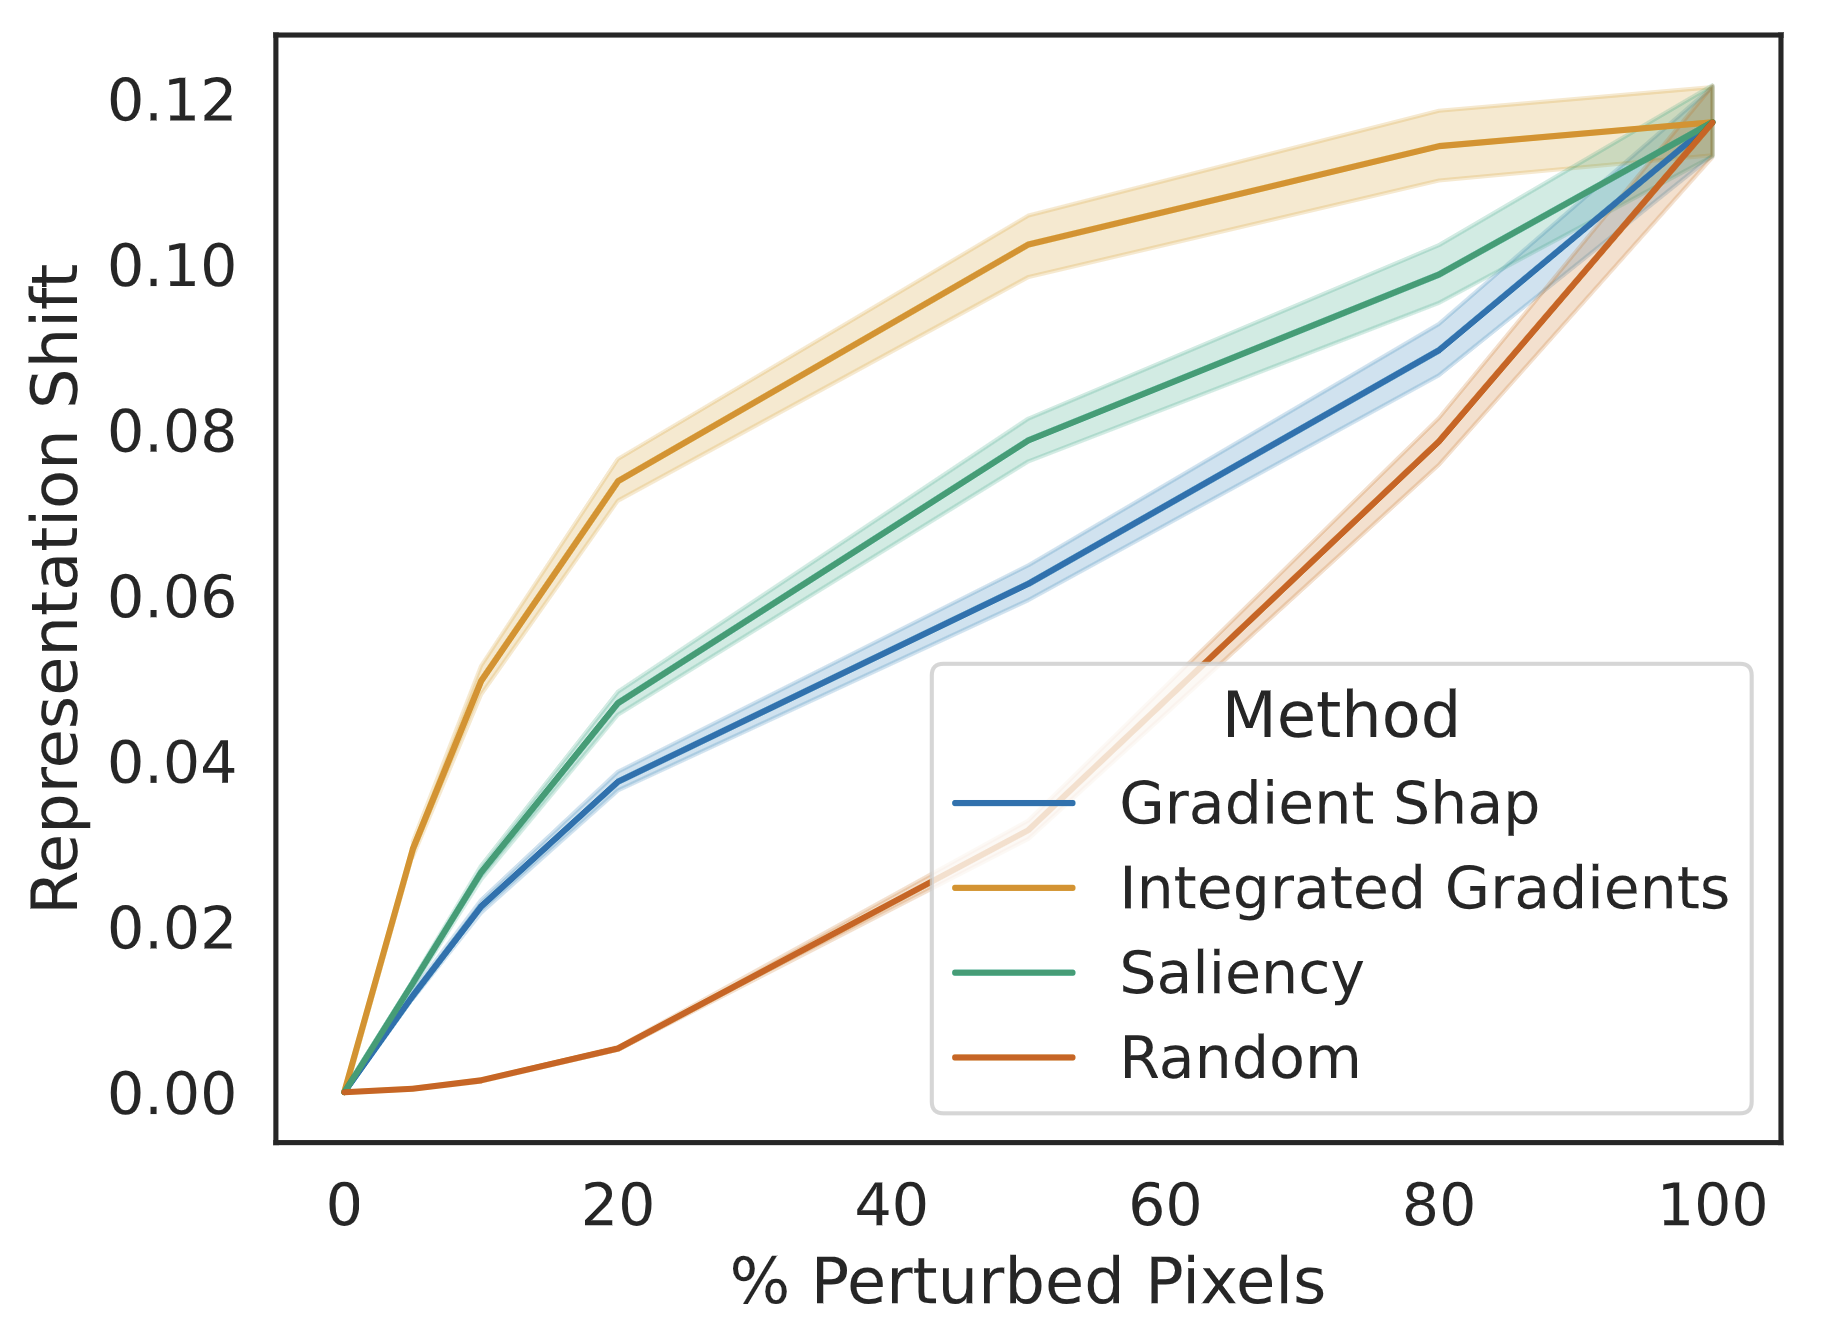
\includegraphics[width=\textwidth]{images/feature_imp/tinyimagenet.png}
            \caption{Tiny ImageNet}\label{fig:tinyimgnet}
        \end{subfigure}
        \begin{subfigure}[b]{0.24\linewidth}
            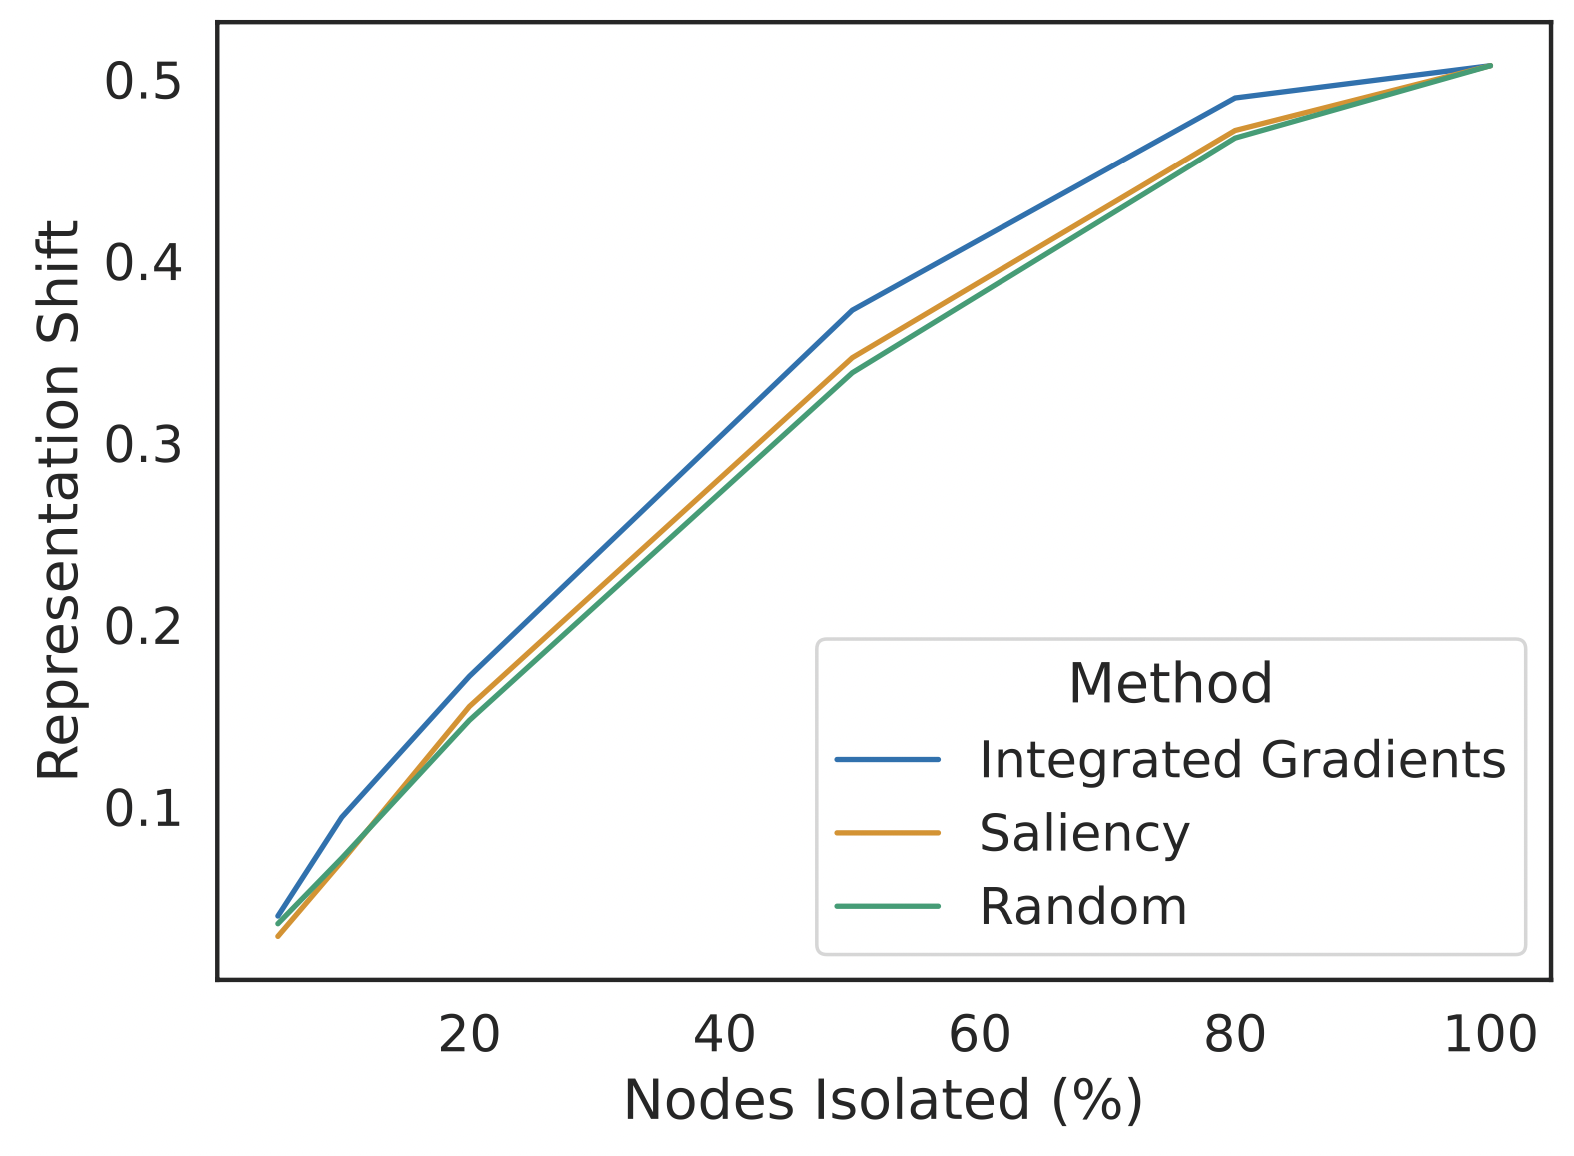
\includegraphics[width=\textwidth]{images/feature_imp/cora.png} 
            \caption{Cora}\label{fig:cora}
        \end{subfigure}
        \begin{subfigure}[b]{0.24\linewidth}
            \includegraphics[width=\textwidth]{images/example_imp/imagenet_200_class.png}
            \caption{Tiny ImageNet}\label{fig:tinyimgnetce}
        \end{subfigure}
        \begin{subfigure}[b]{0.24\linewidth}
            \includegraphics[width=\textwidth]{images/example_imp/agnews.png} 
            \caption{AGNews}\label{fig:agnews}
        \end{subfigure}
        \caption{ Figures \ref{fig:tinyimgnet} and \ref{fig:cora} are for Feature Importance and Figures \ref{fig:tinyimgnetce} and \ref{fig:agnews} are for Example Importance on additional datasets.}
        \label{fig:prob1_6_2}
    \end{minipage}%
    % \begin{minipage}{0.5\textwidth}
    %     \centering
    %     \begin{subfigure}[b]{0.48\linewidth}
    %         \includegraphics[width=\textwidth]{images/example_imp/imagenet_200_class.png}
    %         \caption{Tiny ImageNet}\label{fig:tinyimgnetce}
    %     \end{subfigure}
    %     \begin{subfigure}[b]{0.48\linewidth}
    %         \includegraphics[width=\textwidth]{images/example_imp/agnews.png} 
    %         \caption{AGNews}\label{fig:agnews}
    %     \end{subfigure}
    %     \caption{Example Importance for OOD$^\dagger$ Datasets}
    %     \label{fig:prob1_6_1}
    % \end{minipage}
\end{figure}

% \blfootnote{$^\dagger$OOD stands for Out Of Distribution.}

% \ref{claim3} is not necessarily true for all models
% We examine whether by using prior knowledge in our VAE models, the disentanglement factor ($\beta$)  helps  the saliency maps (SM) to pay attention to different parts of the input image; thus becoming more interpretable.
\subsubsection{Challenging the Generalizability of \ref{claim3} with Attribution Priors}\label{sec:result3extra}
As discussed in Section \ref{sec:expsetup}, we aim to improve the interpretability of d-VAE models ($\beta$ and TC) using pixel attribution prior. 
In Figure \ref{fig:mnistvaeboxattrpr}, we see the PCCs between SM of different latent units for the two d-VAE models with attribution priors. In this case, with the increase in $\beta$, there is a clear decrease in the correlation between the latent units' SM. This denotes that latent units pay attention to different parts of the input image as we increase $\beta$. We see the same observations for different values of $\lambda$ in Figure \ref{fig:attrpriorsboxplts}.
In conclusion, d-VAEs with attribution prior identify better the role of each latent unit with their SM (\textbf{the interpretability is not hard anymore}). Furthermore, the interpretability of SM is related to the strength of the disentanglement between the units. 
Thus, given our experiments, \textbf{\ref{claim3} is not reproducible for \underline{these two d-VAE models} when we use attribution priors}. We present a qualitative analysis with attribution priors in Appendix Section \ref{app:qualresult3extra}.


\section{Discussion}
\label{sec:discussion}
% Give your judgment on if your experimental results support the claims of the paper. Discuss the strengths and weaknesses of your approach - perhaps you didn't have time to run all the experiments, or perhaps you did additional experiments that further strengthened the claims in the paper.
% 1. we say that we support almost all the claims, except for the trend of cifar, give reason for it.
% in conclusion, we support the claims

% 2. Additional experiments and their claims 

% 3. Recommendations for author 

We reproduce the same results for the  experiments as the original paper except for the result of  CIFAR-10's experiment (Section \ref{sssec:result1}). We communicated with the authors about this discrepancy. They hinted that it may be due to the difference in model weights for SimCLR. However, due to time and resource constraints, we could not investigate further by running more explorative experiments. We conclude that \ref{claim1} is partially reproducible while others are completely reproducible. 
\\
\\
We now discuss the reproducibility of claims for our additional experiments. \ref{claim1} is not reproducible  for graphs, discussed in Section \ref{sec:result1extra}. \ref{claim2} is reproducible for Tiny ImageNet and text-based AGNews dataset, discussed in Section \ref{sec:result2extra}. We find that when we use attribution priors, \ref{claim3} is not generalizable to all d-VAE models since it is not reproducible for the two d-VAE models ($\beta$ and TC), as discussed in Section \ref{sec:result3extra}. 
\\
\\
Through our additional experiments, we realize that there is scope for future work in the following areas. The first one is the extension of feature-importance methods to explain spatial attributes of graphs (edges, subgraphs). The second one is improving the interpretability of saliency maps for d-VAE models other than $\beta$-VAE and TC-VAE, by the use of attribution prior. Lastly, we note that running the Influence function (Section \ref{ex_theory}) to obtain an estimation of a shift in loss is time-consuming when we have large amounts of training samples (18 hours for $N=1000$ time-series training samples). We also observe that the DKNN method gives a better (if not the best) measure of importance scores while being computationally fast and we suggest using the same method for further downstream tasks in future works. 
Overall, the experiments in the original paper are reproduced, and their main claims seem reasonably substantiated but could benefit from additional evidence in future research.



\subsection{What was easy}
The authors have significantly helped us to understand the problem, the suggested solution for the problem, and their claims, by providing a well-structured paper that includes detailed appendices consisting of mathematical proofs, implementation details, and experiments. It was easy to begin experimenting with their proposed methods, since the implementations provided are well-organized and fairly documented,  with clear instructions on how to get started. 
% Give your judgement of what was easy to reproduce. Perhaps the author's code is clearly written and easy to run, so it was easy to verify the majority of original claims. Or, the explanation in the paper was really easy to follow and put into code. 

% Be careful not to give sweeping generalizations. Something that is easy for you might be difficult to others. Put what was easy in context and explain why it was easy (e.g. code had extensive API documentation and a lot of examples that matched experiments in papers). 

\subsection{What was difficult}
% List part of the reproduction study that took more time than you anticipated or you felt were difficult. 

% Be careful to put your discussion in context. For example, don't say "the maths was difficult to follow", say "the math requires advanced knowledge of calculus to follow". 

% Also, some of the methodologies for explaining graphs are (i) for supervised setting \citep{gnnpaper} and (ii) are currently in development \citep{torchgeo:online}.  This issue persisted when computing feature importance scores for text explainability.

% For text and graph explainability, we found it difficult to compute feature importance scores.

We found it difficult to extrapolate feature AMs to additional datasets. For example, the majority of the methodologies for explaining graphs are (i) for supervised setting \citep{gnnpaper} and (ii) the unsupervised setting of them is currently in development \citep{torchgeo:online}. While computing feature importance scores for Text Explainability, we encountered an issue where the use of the embedding layer in our Text Autoencoder (see Appendix \ref{appendix:textexplain}) was incompatible with available AMs within Captum \citep{Captum:online}. Also, we couldn't identify the right configurations for the CIFAR-10 experiment to reproduce similar trends as the original paper for feature importance.

\subsection{Communication with original authors}
% Document the extent of (or lack of) communication with the original authors. To make sure the reproducibility report is a fair assessment of the original research we recommend getting in touch with the original authors. You can ask authors specific questions, or if you don't have any questions you can send them the full report to get their feedback before it gets published. 
We reached out to the authors once about our queries regarding the discrepancy in results for feature importance for the CIFAR-10 experiment and to understand the assumptions and contexts of some sub-claims in the paper. We received a prompt response which satisfied most of our questions. 
